% Section 6 --- The audit result
% author had already escaped 3b\_EHq; no smart-quotes present). Table 1 is
% built separately at tables/table1_branch_disposition.tex (non-floating
% longtable) and \input here, in-section, immediately after the
% label-definition paragraph. Every number was verified against the lock and
% the v04 verdict JSONs.
\section{The audit result}\label{sec:result}

The v0.4 audit is presented as method-plus-audited-examples, not a fifteen-branch certification: it does not validate Widom adsorption prediction in general, but it establishes a small set of clean controls and audit-corrected examples within their stated bands and documents the defects the audit caught. The strict result is two passes out of fifteen verdict-affecting branches: the clean MFI + Ar control, branch 6c, and the UiO-66 + CO\(_2\) branch under genuine UFF, branch 3a (Figure~\ref{fig:strict}). The Tier-B physical-accuracy result is five passes out of fifteen: 6c, 3a, the HKUST-1 + CO\(_2\) branch 2a (genuine UFF), the Si-CHA + CO\(_2\) Bai 2013 branch 4c, and the UiO-66 + CO\(_2\) explicit-hydrogen, Yang-charge branch 3b\_EHq (Figure~\ref{fig:disposition}).

Table~\ref{tab:branch-disposition} gives the branch-level disposition. It should be read as a map of causes, not as a leaderboard. A strict pass means that both \(K_H\) and \(Q_{st}\) lie inside the tight regression band. A Tier-B pass means that the branch fails the strict gate but remains inside the broader physical-accuracy band justified for that system. A force-field disagreement means that the energy model does not reproduce the selected reference. A reference-observable mismatch means that the literature number and the Widom zero-coverage quantity are not the same observable. A structural blocker means that the simulated structure is missing, incomplete, or not the experimental material. An ensemble or method mismatch means that the calculation samples a different configuration space from the experiment.

% Table 1 --- branch-level disposition. Built 2026-06-09.
% tables/table1_branch_disposition.source.md. Non-headline deltas were
% re-read directly from evidence/v04_two_tier/verdicts/*.json (and 6e from
% evidence/v04_6e_bai_2013/verdicts/6e.json); 6c/4c/3b_EHq from the lock.
% NON-FLOATING longtable. Do not convert to table[t]. Label: tab:branch-disposition.
{\scriptsize
\setlength{\tabcolsep}{3pt}
\renewcommand{\arraystretch}{1.25}
\begin{longtable}{@{}>{\raggedright\arraybackslash}p{0.072\textwidth}>{\raggedright\arraybackslash}p{0.105\textwidth}>{\raggedright\arraybackslash}p{0.225\textwidth}r r >{\raggedright\arraybackslash}p{0.10\textwidth}>{\raggedright\arraybackslash}p{0.165\textwidth}@{}}
\caption{Branch-level disposition of the v0.4 audit. The headline strict-pass
denominator is fifteen verdict-affecting scalar branches. The UiO-66 3b family
is shown in three force-field variants for scientific transparency but is
counted according to the locked v0.4 disposition; branch 5b is shown as
method-blocked and is not scored as a scalar $K_H$/$Q_{st}$ pass or fail. The
Tier-A strict passes are 6c and 3a. The Tier-B physical-accuracy passes are 6c,
3a, 2a, 4c, and 3b\_EHq. Branches 2a and 3a are the v0.4.2 genuine-UFF rebuild
(superseded as-locked deviations in parentheses); 4c is reported on RASPA3 as
Tier-B, its strict label being engine-marginal. Branch identifiers are internal
locked-recipe labels, retained only to keep the table traceable to the repository
and its evidence JSON; for example 6c = all-silica MFI + Ar, 3a = UiO-66 +
CO\textsubscript{2} (genuine UFF), 2a = HKUST-1 + CO\textsubscript{2} (genuine
UFF), 4c = Si-CHA + CO\textsubscript{2} (Bai 2013 control), and 3b\_EHq = UiO-66 +
CO\textsubscript{2} (Maia 2023 explicit-hydrogen, charged).}\label{tab:branch-disposition}\\
\toprule
Br. & System & Recipe (structure / force field / gas) & $\Delta\log_{10}K_H$ & $\Delta Q_{st}$ & Class & Reason \\
\midrule
\endfirsthead
\multicolumn{7}{@{}l}{\footnotesize\emph{Table~\ref{tab:branch-disposition}, continued}}\\
\toprule
Br. & System & Recipe (structure / force field / gas) & $\Delta\log_{10}K_H$ & $\Delta Q_{st}$ & Class & Reason \\
\midrule
\endhead
\midrule
\multicolumn{7}{@{}r}{\footnotesize\emph{continued on next page}}\\
\endfoot
\bottomrule
\endlastfoot
\multicolumn{7}{@{}l}{\textit{(a) Strict passes}}\\
6c & MFI + Ar & all-silica MFI (Olson 1981 geometry) / Talu--Myers Ar, oxygen-only single-source\cite{Talu2001}; native + RASPA3 & $0.000$ & $-0.73$ & Tier A PASS & clean control, single-source (no Si double-count) \\
3a & UiO-66 + CO\textsubscript{2} & all-silica UiO-66 / genuine UFF framework + DDEC charges / TraPPE-CO\textsubscript{2}; RASPA3 & $+0.086$ & $-0.89$ & Tier A PASS & genuine-UFF rebuild reproduces experiment (v0.4.2; was $-0.802$) \\
\addlinespace[2pt]
\multicolumn{7}{@{}l}{\textit{(b) Tier-B physical passes (Tier A fail)}}\\
2a & HKUST-1 + CO\textsubscript{2} & HKUST-1 / genuine UFF framework + Nazarian DDEC\cite{Nazarian2016ChemMater} / EPM2; RASPA3 & $+0.13$ & $+3.9$ & Tier B PASS & genuine-UFF rebuild; $K_H$ 8.3--10.8 (open-Cu tail); was $-0.759$ \\
4c & Si-CHA + CO\textsubscript{2} & IZA Si-CHA / Bai 2013 TraPPE-zeo / TraPPE-CO\textsubscript{2}\cite{PotoffSiepmann2001AIChE}; native + RASPA3 & $-0.079$ & $+2.24$ & Tier B PASS & cross-engine-audited (native$\leftrightarrow$RASPA3 $\sim$9\%); $Q_{st}$ engine-marginal \\
3b\_EHq & UiO-66 + CO\textsubscript{2} & UiO-66 / Maia 2023 explicit-H + Yang charges / TraPPE & $-0.252$ & $-4.43$ & Tier B PASS & within UiO-66 synthesis-scatter band \\
\addlinespace[2pt]
\multicolumn{7}{@{}l}{\textit{(c) Near-misses by recorded agreement class (Tier A fail)}}\\
3b\_UA & UiO-66 + CO\textsubscript{2} & Maia 2023 united-atom, no charge & $-0.411$ & $-6.09$ & within $2\sigma$ & united-atom under-binds \\
3b\_UAq & UiO-66 + CO\textsubscript{2} & Maia 2023 united-atom + Yang charges & $-0.415$ & $-5.86$ & within $2\sigma$ & united-atom under-binds \\
4a & Si-CHA + CO\textsubscript{2} & TraPPE-zeo + Harris--Yung CO\textsubscript{2}\cite{HarrisYung1995JPC} & $-0.116$ & $+11.74$ & within $2\sigma$ & gas-model-dependent $Q_{st}$ \\
6b & MFI + Kr & Garc\'\i a-P\'erez framework + Talu cross-pair & $+0.071$ & $-4.17$ & within $2\sigma$ & $Q_{st}$ reference is a van't Hoff fit \\
6e & MFI + CH\textsubscript{4} & Bai 2013 TraPPE-zeo + TraPPE-UA CH\textsubscript{4}\cite{MartinSiepmann1998JPCB} & $-0.296$ & $-2.14$ & within $2\sigma$ & TraPPE-zeo/UA under-binds (Shah 2015 agrees)\cite{Shah2015Langmuir} \\
\addlinespace[2pt]
\multicolumn{7}{@{}l}{\textit{(d) Force-field disagreements ($2$--$3\sigma$ tension and $>3\sigma$)}}\\
1c & Mg-MOF-74 + CO\textsubscript{2} & Becker 2018 reduced-LJ (as-run framework = plain UFF + Mg placeholder) & $+0.581$ & $+4.01$ & $2$--$3\sigma$ & audit-caught parameter-substitution defect (see text) \\
1a & Mg-MOF-74 + CO\textsubscript{2} & Lin et al.\ 2014 Buckingham + EPM2\cite{LinMercado2014JCTC} & $+1.765$ & $+8.83$ & $>3\sigma$ & DFT cross-pairs over-bind (no polarisation) \\
1b & Mg-MOF-74 + CO\textsubscript{2} & Dzubak 2012 ($A\,e^{-Br}-C/r^5-D/r^6$)\cite{Dzubak2012NatChem} + TraPPE & $+1.799$ & $+9.55$ & $>3\sigma$ & over-binds vs experiment; parity unresolved \\
1d & Mg-MOF-74 + CO\textsubscript{2} & Mercado 2016 Model 4 (Buckingham + LJ)\cite{Mercado2016JPCC} & $+1.716$ & $+11.84$ & $>3\sigma$ & over-binds open metal site \\
2b & HKUST-1 + CO\textsubscript{2} & Ongari 2017 modified Cu-O(CO\textsubscript{2})\cite{Ongari2017JPCC} & $+1.400$ & $+14.03$ & $>3\sigma$ & over-binds Cu paddle-wheel \\
6a & MFI + CH\textsubscript{4} & Garc\'\i a-P\'erez 2007 + Dubbeldam 2004 UA\cite{Dubbeldam2004UA} & $-0.347$ & $-2.43$ & $>3\sigma$ & united-atom under-binds \\
\addlinespace[2pt]
\multicolumn{7}{@{}l}{\textit{(e) Method-blocked}}\\
5b & Na-Rho + CO\textsubscript{2} & rigid closed-state Widom vs open-state experiment & --- & --- & ensemble mismatch & different partition functions; no scalar pass/fail \\
\end{longtable}
}


\begin{figure}[tbp]
\centering
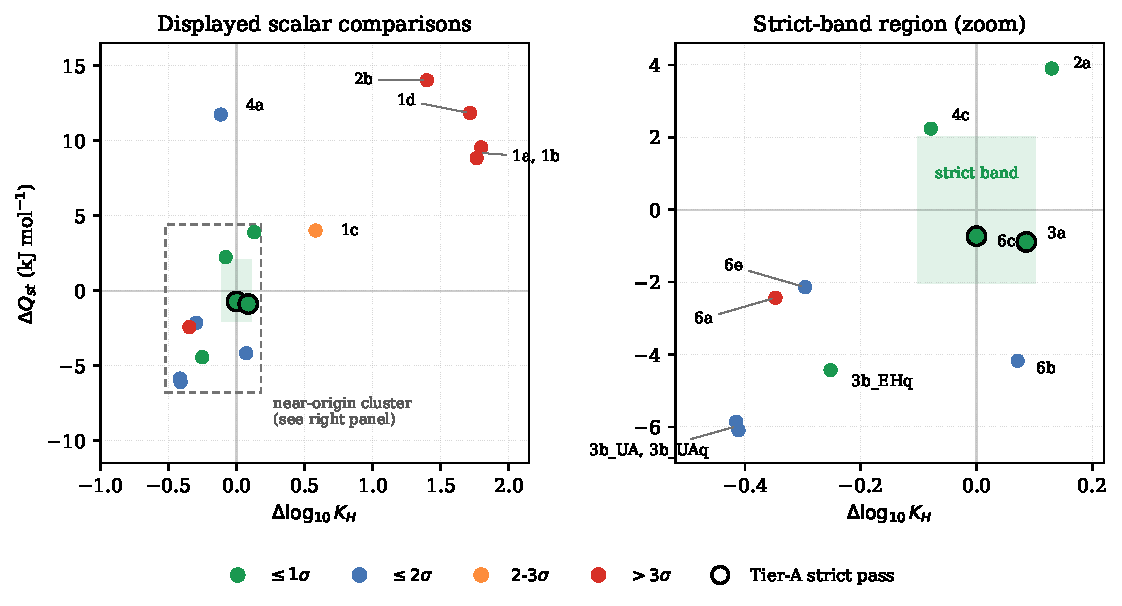
\includegraphics[width=\textwidth]{figures/fig2_strict_result.pdf}
\caption{Strict result. The scalar comparison rows of Table~\ref{tab:branch-disposition} in the deviation plane (\(\Delta\log_{10}K_H\), \(\Delta Q_{st}\)); the shaded box is the Tier-A strict band (\(\pm0.10\), \(\pm2.0\ \mathrm{kJ\,mol^{-1}}\)). Only 6c and 3a (black-edged) fall inside it --- the two-of-fifteen strict result. The right panel zooms on the near-origin region, where 2a, 4c, and 3b\_EHq sit just outside the band as Tier-B passes (3a sits inside, alongside 6c). The UiO-66 3b family is displayed in its three force-field variants; the headline denominator remains the fifteen-branch disposition described in Table~\ref{tab:branch-disposition} and Appendix~\ref{app:branch-table}. Deviations are read from the production runs --- 2a, 3a, and 4c from the v0.4.2 genuine-UFF / cross-engine rebuild; the 6c \(Q_{st}\) deviation is \(-0.73\ \mathrm{kJ\,mol^{-1}}\) (Dunne 1996 reference \(Q_{st}=15.7\ \mathrm{kJ\,mol^{-1}}\)). Branch 5b is method-blocked and is not plotted. Branch codes are internal locked-recipe identifiers; see the reader note in Section~\ref{sec:problem}.}
\label{fig:strict}
\end{figure}

\begin{figure}[tbp]
\centering
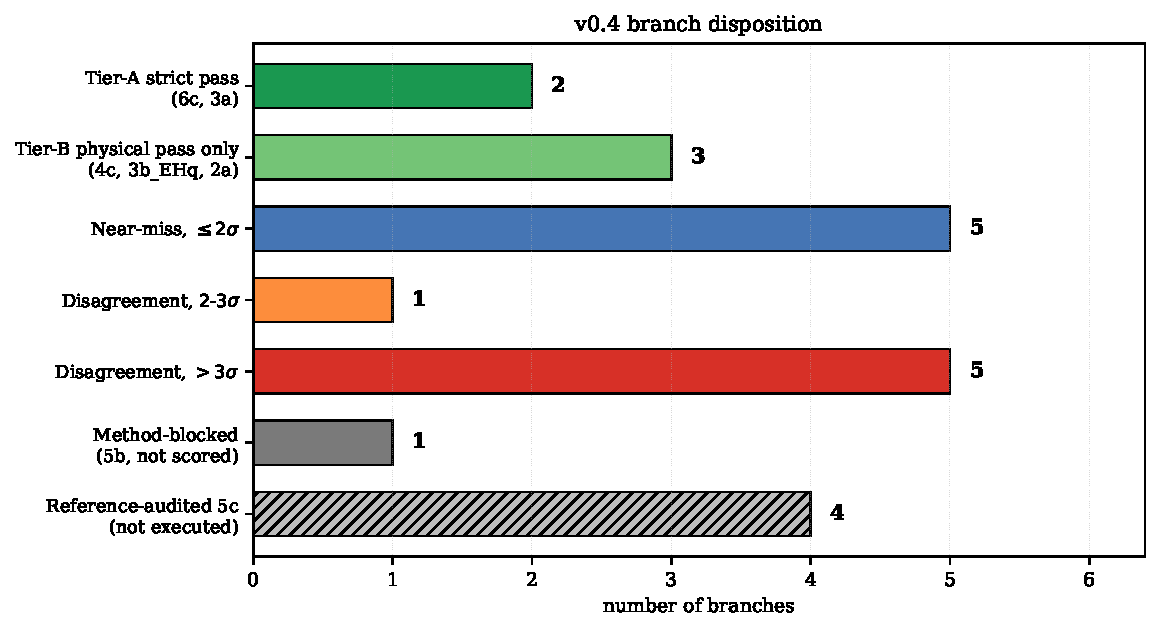
\includegraphics[width=0.80\textwidth]{figures/fig3_branch_disposition.pdf}
\caption{Branch disposition in mutually-exclusive outcome categories. The two Tier-A strict passes (6c, 3a) and the additional Tier-B physical passes (2a, 4c, 3b\_EHq) are the \(2/15\) and \(5/15\) headline; the remaining scalar rows are force-field disagreements and near-misses. The UiO-66 3b family is displayed in its three force-field variants, so the displayed scalar rows total sixteen but are counted as the locked fifteen-branch denominator (see Table~\ref{tab:branch-disposition} and Appendix~\ref{app:branch-table}). Branch 5b is method-blocked and not scalar-scored; the 5c cationic-zeolite targets are reference-audited and not executed. Counts are computed from the audited branch data. Branch codes are internal locked-recipe identifiers; see the reader note in Section~\ref{sec:problem}.}
\label{fig:disposition}
\end{figure}

Two of these branches are deliberate controls. Branch 6c is the simplest: all-silica MFI, argon, no charges, no flexible framework mechanism; it is a Tier-A strict pass cross-confirmed by the native estimator and RASPA3 to \(0.5\%\). Branch 4c is more demanding --- Si-CHA + CO\(_2\), Bai 2013 TraPPE-zeo parameters, electrostatics, and an analytical tail correction --- and is a cross-engine-audited charged control: the native estimator and RASPA3 agree to \(\sim\!9\%\) on \(K_H\) and \(\sim\!1\%\) on \(Q_{st}\), and the result sits inside the experimental window. Its strict-versus-Tier-B verdict is itself engine-dependent --- the \(Q_{st}\) deviation sits on the \(\pm2.0\) boundary (native \(+1.99\), inside; RASPA3 \(+2.24\), outside), so the same recipe is nominally strict on one engine and Tier-B on the other. We therefore report it as Tier-B, and note this as a worked example, on a charged system, of the verdict fragility this harness exists to expose.

The other two passes are audit-caught corrections, not controls. Branches 2a (HKUST-1 + CO\(_2\)) and 3a (UiO-66 + CO\(_2\)) were originally locked as a \(>3\sigma\) and a \(2\)--\(3\sigma\) force-field failure and read as ``UFF under-binds the open metal site.'' That reading was an artifact. The originally-locked recipe routed the MOF framework through a generator that hard-coded a zeolite/cation table and unconditionally stamped \texttt{source="UFF"} on framework atoms that were in fact the Harris-Yung CO\(_2\)-carbon (\(\epsilon = 28.1\) K vs genuine UFF \(52.8\)), TraPPE-zeo oxygen (\(53.0\) vs UFF \(30.2\)), and a wrong-\(\epsilon\) hydrogen --- only the metals were genuine UFF. Corrected to genuine UFF, the aromatic-linker dispersion compensates the genuinely weak UFF open-metal site and both MOFs reproduce experiment: 3a near-exactly (\(\Delta\log_{10}K_H = +0.086\), \(\Delta Q_{st} = -0.89\ \mathrm{kJ\,mol^{-1}}\); Tier-A strict), and 2a slightly over (\(K_H\) in the range \(8.3\)--\(10.8\ \mathrm{mol\,kg^{-1}\,bar^{-1}}\), reported as a range because of the open-Cu deep-well sampling tail; \(\Delta Q_{st} = +3.9\ \mathrm{kJ\,mol^{-1}}\); Tier-B). Both are reported from RASPA3 only: the native estimator cannot corroborate them because its charged-Ewald path shows a large, not-yet-root-caused discrepancy against RASPA3 on these MOF cells (Section~\ref{sec:controls}). This is a second worked example of the paper's own thesis --- a generator silently substituting parameters under a false label, caught by the harness --- parallel to the 6c silicon double-count. The originally-locked (buggy) deviations, \(\Delta\log_{10}K_H = -0.759\) (2a) and \(-0.802\) (3a), are retained in the case matrix as the documented superseded case.

A further Tier-B pass is different in kind again. Branch 3b\_EHq, UiO-66 + CO\(_2\) under the Maia 2023 explicit-hydrogen, Yang-charge variant, gives \(K_H = 2.87 \pm 0.094\ \mathrm{mol\,kg^{-1}\,bar^{-1}}\) and \(Q_{st} = 22.07 \pm 0.13\ \mathrm{kJ\,mol^{-1}}\), corresponding to \(\Delta \log_{10}K_H = -0.252\) and \(\Delta Q_{st} = -4.43\ \mathrm{kJ\,mol^{-1}}\). That is outside the strict band, but inside the physical-accuracy band defined for UiO-66. This is why it is not counted as a strict pass but is counted as a Tier-B physical pass.

Several branches are near-misses rather than clear successes. The united-atom UiO-66 variants, the MFI + CH\(_4\) Bai branch \cite{Hufton1993AIChE}, the Si-CHA Harris-Yung branch, and the MFI + Kr branch \cite{GoldenSircar1994JCIS} do not pass the strict gate. Some remain within the recorded two-sigma agreement class --- a diagnostic classification of the \(K_H\) log-space deviation, not a Tier-A pass criterion --- and several failures are dominated by \(Q_{st}\) rather than \(K_H\). These branches are useful because they show where a recipe is close enough to be scientifically informative but not close enough to be used as a strict validation point.

The strongest disagreements occur in the open-metal-site systems. Mg-MOF-74 + CO\(_2\) \cite{Mason2011EES,Britt2009PNAS,Queen2011JPCC,Wu2010JPCL,Simmons2011EES,Queen2014ChemSci} and HKUST-1 + CO\(_2\) \cite{Grajciar2011JPCC} expose a limitation of non-polarisable or simplified pairwise force fields at strong binding sites. Some branches over-bind and others under-bind, depending on the force-field family, but the common point is that the simple recipe does not transfer cleanly to the chemistry of the exposed metal site. The harness does not repair that failure; it names it.

The Na-Rho branch is a different case. Branch 5b is not scored as a scalar \(K_H/Q_{st}\) pass or fail. Rigid closed-state Widom samples a closed framework partition function, while the experimental adsorption observable involves a trapdoor opening process. The calculation and experiment are therefore not the same statistical-mechanical object. The site-geometry comparison can still be audited separately, but the scalar zero-coverage comparison is method-blocked.

The 5c cationic-zeolite family is also deliberately not treated as a hidden validation. Na-ZK-5, Zeolite 5A, Zeolite 13X, and Zeolite 4A have reference information recorded, but they require cation-containing structures and locked cation force-field and charge models before execution. Until those ingredients are supplied, they are reference-audited targets, not completed branches, and they do not validate Na-Rho.

The result is therefore smaller and more useful than a simple pass count. The atlas does not say that two passes make a general adsorption predictor. It says which recipes currently reproduce experiment, which recipes fail by force-field transferability, which are blocked by missing structures or incompatible references, and which are outside the rigid-Widom observable altogether. That is the value of the audit.

\FloatBarrier
